\documentclass{article}

\usepackage[utf8]{inputenc}
\usepackage{graphicx}
\usepackage{amsmath}
\usepackage{hyperref}
\usepackage{tikz}
\usetikzlibrary{positioning,shapes.geometric}

\author{Equipo 32: \\
Ismael Rufino Grajeda Marin \\
xxx\\
xxx\\
xxx\\
}
\date{2 de marzo de 2024}

\begin{document}

\noindent
\begin{minipage}{0.3\textwidth}
    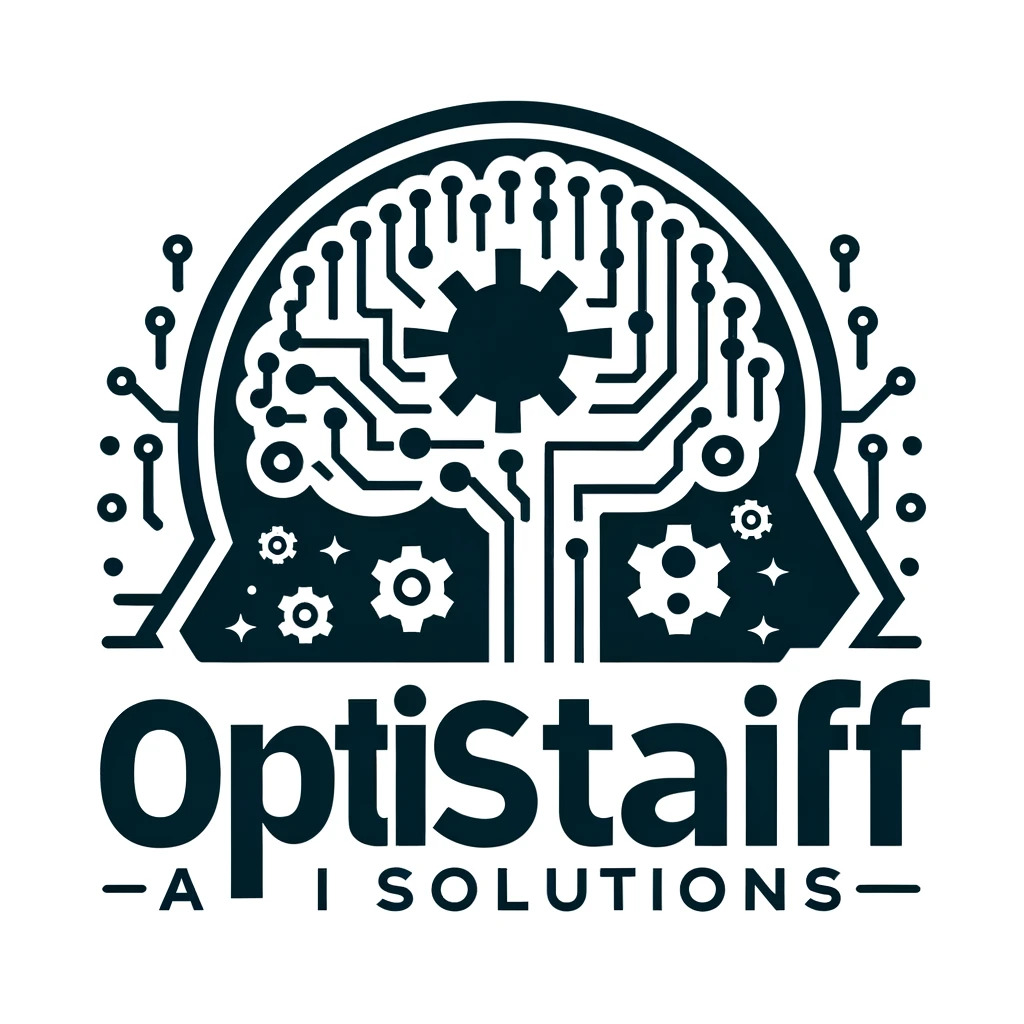
\includegraphics[width=\textwidth]{logo_empresa.jpeg}
\end{minipage}%
\begin{minipage}{0.7\textwidth}
    {\Large \textbf{IntelliStaff AI Solutions}}\\[1ex]
    {\large Potenciando Proyectos}
\end{minipage}

\bigskip 

\section{Misión}
Proporcionar soluciones avanzadas de inteligencia artificial para optimizar el tiempo del personal, mejorando significativamente la eficiencia y productividad de nuestros clientes a través de la innovación tecnológica y un profundo entendimiento de las necesidades de gestión de recursos humanos.

\section{Visiones}
\subsection{Visión a Corto Plazo}
Establecer a OptiStaff AI Solutions como el referente en soluciones de optimización de personal en el sector de la construcción, demostrando mejoras tangibles en eficiencia y productividad en todos los proyectos implementados.

\subsection{Visión a Mediano Plazo}
Diversificar nuestras soluciones de optimización de personal utilizando IA en diferentes industrias, adaptando nuestros algoritmos para satisfacer una variedad de necesidades laborales y estableciendo alianzas estratégicas para ampliar nuestro alcance de mercado.

\subsection{Visión a Largo Plazo}
Ser líderes globales en la innovación de soluciones de inteligencia artificial para la gestión de recursos humanos, transformando la forma en que las organizaciones optimizan sus equipos de trabajo, con un enfoque en sostenibilidad, inclusión y desarrollo de talento.



\begin{abstract}
    El objetivo de este estudio es desarrollar e implementar un sistema de gestión de proyectos que utilice inteligencia artificial para optimizar la selección de equipos de trabajo. Mediante el uso de un modelo de redes neuronales, el sistema calculará el porcentaje de éxito de cada equipo potencial, basándose en sus perfiles y el perfil del proyecto, facilitando así la toma de decisiones en la asignación de recursos humanos.
\end{abstract}

\section{Introducción}
En el contexto actual, muchas organizaciones enfrentan desafíos significativos en la gestión eficiente de su personal. La asignación de tareas a menudo no toma en cuenta de manera óptima las habilidades, experiencia y rendimientos anteriores de los trabajadores, lo que puede resultar en asignaciones ineficientes, desperdicio de talento y recursos, y en última instancia, en la disminución de la productividad y eficiencia de los proyectos. Este problema se ve agravado por la falta de herramientas adecuadas que permitan una gestión dinámica y adaptativa del personal, capaz de responder rápidamente a las cambiantes necesidades de los proyectos y a las variaciones en la disponibilidad y capacidades del personal.

En este contexto, nuestro proyecto, OptiStaff AI Solutions, propone un sistema de gestión de proyectos que incorpora inteligencia artificial para abordar estos desafíos. Nuestro sistema está diseñado para optimizar la asignación de tareas y mejorar la eficiencia general de la gestión de recursos humanos, utilizando un modelo de redes neuronales para predecir el éxito del equipo y seleccionar el mejor equipo de trabajo para cada proyecto, de manera similar a sistemas como Asana o Jira, pero con capacidades avanzadas de inteligencia artificial.

\section{Hipótesis}
La hipótesis de este proyecto es que la implementación de un sistema de gestión de proyectos con inteligencia artificial, específicamente a través de un modelo de redes neuronales, mejorará significativamente la eficiencia y productividad en la asignación de tareas y la selección de equipos de trabajo. Se espera que este sistema permita una asignación más precisa de los recursos humanos, basada en las habilidades y experiencias de los trabajadores, así como en las necesidades específicas de cada proyecto, resultando en una mejora tangible en la ejecución y el éxito de los proyectos.

\section{Objetivos}
    \subsection{Objetivo General}
    Desarrollar e implementar un sistema de gestión de proyectos que integre inteligencia artificial para la selección óptima de equipos de trabajo, basándose en el análisis de perfiles y la compatibilidad con el proyecto.

    \subsection{Objetivos Específicos}
    \begin{itemize}
        \item Diseñar la arquitectura del sistema de gestión de proyectos que incorpore componentes de inteligencia artificial.
        \item Desarrollar un modelo de redes neuronales que evalúe la compatibilidad entre los perfiles de los trabajadores y los requisitos del proyecto.
        \item Implementar el sistema y validar su eficacia en la selección de equipos de trabajo y la predicción del éxito del proyecto.
        \item Capacitar al personal en el uso del sistema y en la interpretación de los resultados proporcionados por el modelo de inteligencia artificial.
    \end{itemize}


    \section{Metas e Indicadores}
    Para cada objetivo específico, se han establecido las siguientes metas e indicadores para evaluar el logro de estas metas:

    \subsection{Metas e Indicadores para el Diseño de la Arquitectura del Sistema}
    \textbf{Meta:} Diseñar una arquitectura de sistema que integre componentes de inteligencia artificial de manera eficiente.
    \begin{itemize}
        \item \textbf{Indicador:} Compleción del diseño de la arquitectura del sistema en un plazo de 2 meses.
        \item \textbf{Indicador:} Integración exitosa de al menos dos componentes de inteligencia artificial en la arquitectura del sistema.
    \end{itemize}

    \subsection{Metas e Indicadores para el Desarrollo del Modelo de Redes Neuronales}
    \textbf{Meta:} Desarrollar un modelo de redes neuronales que evalúe la compatibilidad entre perfiles de trabajadores y requisitos del proyecto.
    \begin{itemize}
        \item \textbf{Indicador:} Precisión del modelo de redes neuronales superior al 80\% en la evaluación de compatibilidad.
        \item \textbf{Indicador:} Finalización del desarrollo del modelo en un plazo de 4 meses.
    \end{itemize}

    \subsection{Metas e Indicadores para la Implementación y Validación del Sistema}
    \textbf{Meta:} Implementar y validar el sistema para asegurar su eficacia en la selección de equipos de trabajo y predicción del éxito del proyecto.
    \begin{itemize}
        \item \textbf{Indicador:} Implementación exitosa del sistema en el entorno de prueba en un plazo de 6 meses.
        \item \textbf{Indicador:} Al menos un 90\% de satisfacción en la evaluación de usuarios durante la fase de prueba.
    \end{itemize}

    \subsection{Metas e Indicadores para la Capacitación del Personal}
    \textbf{Meta:} Capacitar al personal en el uso del sistema y en la interpretación de los resultados proporcionados por el modelo de inteligencia artificial.
    \begin{itemize}
        \item \textbf{Indicador:} Al menos el 80\% del personal encargado de la gestión de proyectos capacitado en el uso del sistema en un plazo de 8 meses.
        \item \textbf{Indicador:} Al menos el 75\% de comprensión en la interpretación de los resultados del modelo de inteligencia artificial según evaluaciones post-capacitación.
    \end{itemize}


    \section{Marco Teórico}
    El desarrollo de sistemas de gestión de proyectos que integran inteligencia artificial es un campo en crecimiento. La incorporación de modelos de redes neuronales para la selección de equipos de trabajo se basa en la capacidad de estas técnicas para procesar y analizar grandes cantidades de datos, identificando patrones y realizando predicciones con alta precisión.
    
    En el contexto de la gestión de proyectos, la inteligencia artificial puede utilizarse para evaluar la compatibilidad entre los perfiles de los trabajadores y los requisitos específicos de un proyecto, optimizando así la asignación de recursos humanos. Este enfoque no solo mejora la eficiencia del proceso de selección de equipos, sino que también aumenta las probabilidades de éxito del proyecto al garantizar una mayor cohesión y complementariedad entre los miembros del equipo.
    
    La implementación de sistemas de gestión de proyectos estilo Asana o Jira con capacidades de inteligencia artificial representa un avance significativo en la forma en que las empresas organizan y ejecutan sus proyectos, permitiendo una toma de decisiones más informada y basada en datos.
    
    \subsection{Revisión de la Literatura}
    La literatura sobre la aplicación de inteligencia artificial en la gestión de proyectos es extensa. Por ejemplo, estudios como el de Smith y Lamsal (2018) han demostrado la eficacia de los algoritmos de aprendizaje automático en la predicción del éxito de los proyectos y la asignación óptima de recursos. Además, investigaciones como la de Johnson y Zhang (2019) han explorado el uso de redes neuronales para mejorar la planificación y ejecución de proyectos en entornos complejos.
    
    \subsection{Soluciones Previas}
    En el mercado actual, existen varias soluciones que incorporan inteligencia artificial para la gestión de proyectos. Por ejemplo, la plataforma Trello utiliza algoritmos de aprendizaje automático para sugerir acciones y prioridades basadas en el comportamiento del usuario. Asimismo, la herramienta Forecast utiliza inteligencia artificial para proporcionar estimaciones precisas de tiempo y recursos necesarios para completar proyectos.
    

\section{Metodología}
    La metodología empleada para el desarrollo del sistema de gestión de proyectos con inteligencia artificial se basará en un enfoque iterativo y ágil. Esto permitirá una adaptación continua del sistema a medida que se avance en su implementación y se obtengan retroalimentaciones.

    \subsection{Diseño del Experimento}
        Para probar la hipótesis de que la implementación de un sistema de gestión de proyectos con inteligencia artificial mejorará significativamente la eficiencia y productividad en la asignación de tareas y la selección de equipos de trabajo, se diseñará un experimento que compare el rendimiento del sistema propuesto con un sistema de gestión de proyectos tradicional.

        \textbf{Configuración del Experimento:}
        \begin{itemize}
            \item Se seleccionarán dos grupos de proyectos similares en términos de complejidad y requisitos de recursos humanos.
            \item Un grupo utilizará el sistema de gestión de proyectos con inteligencia artificial, mientras que el otro utilizará un sistema tradicional.
            \item Se medirá el tiempo de finalización, la calidad del trabajo y la satisfacción del equipo en ambos grupos.
        \end{itemize}

        \textbf{Métricas de Evaluación:}
        \begin{itemize}
            \item \textbf{Eficiencia:} Tiempo promedio de finalización de los proyectos.
            \item \textbf{Calidad:} Número de errores o problemas reportados durante y después de la finalización del proyecto.
            \item \textbf{Satisfacción del Equipo:} Encuestas de satisfacción realizadas a los miembros del equipo de cada proyecto.
        \end{itemize}

        \textbf{Análisis de Resultados:}
        Se utilizarán pruebas estadísticas para determinar si las diferencias observadas en las métricas de evaluación son significativas. Se espera que el sistema de gestión de proyectos con inteligencia artificial muestre una mejora en la eficiencia y la calidad del trabajo, así como una mayor satisfacción del equipo en comparación con el sistema tradicional.

    \subsection{Desarrollo del Modelo de Redes Neuronales}
    Se utilizarán técnicas de aprendizaje automático para desarrollar un modelo de redes neuronales capaz de evaluar la compatibilidad entre los perfiles de los trabajadores y los requisitos del proyecto. Este modelo se entrenará con datos históricos de proyectos anteriores y se validará con conjuntos de datos de prueba para garantizar su precisión.

    \subsection{Integración del Modelo en el Sistema de Gestión de Proyectos}
    Una vez desarrollado y validado el modelo, se integrará en el sistema de gestión de proyectos. Se establecerán interfaces de usuario intuitivas para permitir a los gestores de proyectos ingresar los datos del proyecto y obtener recomendaciones sobre la selección de equipos.

    \subsection{Pruebas y Validación}
    Se realizarán pruebas exhaustivas del sistema para asegurar su funcionamiento correcto y la precisión de las recomendaciones proporcionadas por el modelo de inteligencia artificial. Esto incluirá pruebas de funcionalidad, pruebas de usabilidad y pruebas de rendimiento.

    \subsection{Capacitación y Despliegue}
    Se proporcionará capacitación al personal encargado de la gestión de proyectos para asegurar un uso eficiente del sistema. Finalmente, se desplegará el sistema en el entorno operativo de la empresa y se monitoreará su rendimiento para realizar ajustes y mejoras continuas.


    \section{Cronograma y Presupuesto}
    La implementación del sistema de gestión de proyectos con inteligencia artificial se llevará a cabo en un periodo de nueve meses, dividido en distintas etapas:
    
   

    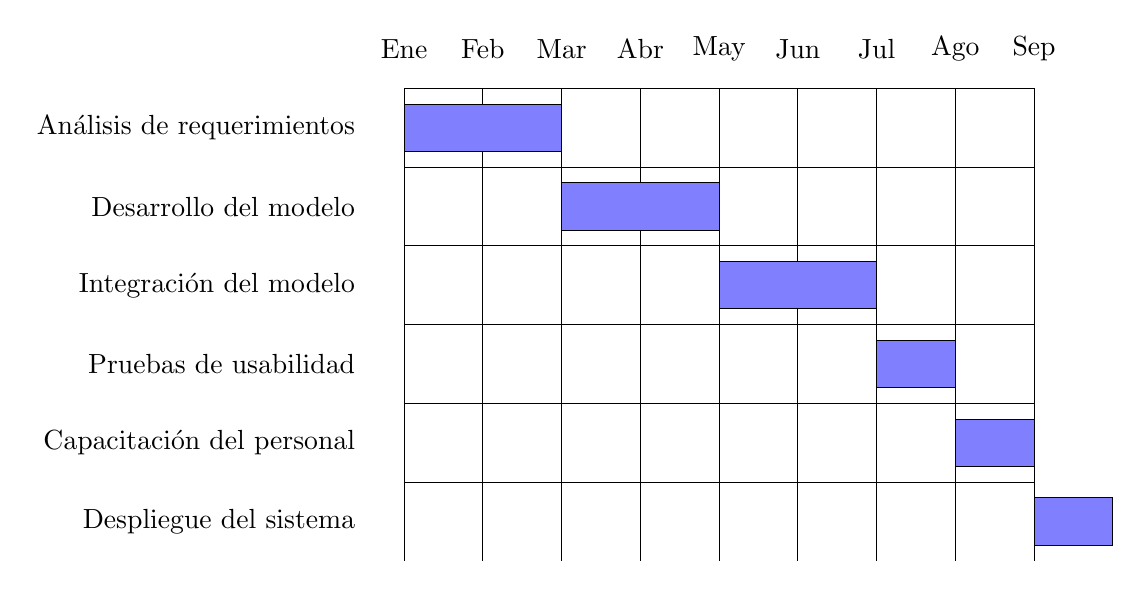
\begin{tikzpicture}[x=1cm, y=1cm, node distance=0.5cm]
        % Draw vertical lines for each month
        \foreach \x in {1,...,9} {
            \draw (\x, 0) -- (\x, -6);
        }
        % Draw horizontal lines for each task
        \foreach \y in {0,...,-5} {
            \draw (1, \y) -- (9, \y);
        }
        % Labels for months
        \foreach \x/\month in {1/Ene, 2/Feb, 3/Mar, 4/Abr, 5/May, 6/Jun, 7/Jul, 8/Ago, 9/Sep} {
            \node at (\x, 0.5) {\month};
        }
        % Labels and bars for tasks
        \node[align=left, anchor=east] at (0.5, -0.5) {Análisis de requerimientos};
        \draw[fill=blue!50] (1, -0.8) rectangle (3, -0.2);
        \node[align=left, anchor=east] at (0.5, -1.5) {Desarrollo del modelo};
        \draw[fill=blue!50] (3, -1.8) rectangle (5, -1.2);
        \node[align=left, anchor=east] at (0.5, -2.5) {Integración del modelo};
        \draw[fill=blue!50] (5, -2.8) rectangle (7, -2.2);
        \node[align=left, anchor=east] at (0.5, -3.5) {Pruebas de usabilidad};
        \draw[fill=blue!50] (7, -3.8) rectangle (8, -3.2);
        \node[align=left, anchor=east] at (0.5, -4.5) {Capacitación del personal};
        \draw[fill=blue!50] (8, -4.8) rectangle (9, -4.2);
        \node[align=left, anchor=east] at (0.5, -5.5) {Despliegue del sistema};
        \draw[fill=blue!50] (9, -5.8) rectangle (10, -5.2);
    \end{tikzpicture}
    
    
    El presupuesto estimado para el proyecto es de \$200,000.00 USD, que incluye los costos de desarrollo del software, pruebas, capacitación del personal y despliegue del sistema. Este presupuesto se distribuirá de la siguiente manera:
    
   
    \begin{enumerate}
        \item \textbf{Mes 1-2: Análisis de requerimientos y diseño preliminar del sistema.}
        \begin{itemize}
            \item \textbf{Entregables:} Documento de requerimientos, bocetos del diseño del sistema.
            \item \textbf{Costo:} \$20,000.00 USD
        \end{itemize}
        \item \textbf{Mes 3-4: Desarrollo del modelo de redes neuronales y pruebas iniciales.}
        \begin{itemize}
            \item \textbf{Entregables:} Modelo de redes neuronales desarrollado, informe de pruebas iniciales.
            \item \textbf{Costo:} \$40,000.00 USD
        \end{itemize}
        \item \textbf{Mes 5-6: Integración del modelo en el sistema de gestión de proyectos y pruebas de funcionalidad.}
        \begin{itemize}
            \item \textbf{Entregables:} Sistema de gestión de proyectos con el modelo integrado, informe de pruebas de funcionalidad.
            \item \textbf{Costo:} \$30,000.00 USD
        \end{itemize}
        \item \textbf{Mes 7: Pruebas de usabilidad y ajustes del sistema.}
        \begin{itemize}
            \item \textbf{Entregables:} Informe de pruebas de usabilidad, sistema ajustado.
            \item \textbf{Costo:} \$20,000.00 USD
        \end{itemize}
        \item \textbf{Mes 8: Capacitación del personal y preparación para el despliegue.}
        \begin{itemize}
            \item \textbf{Entregables:} Material de capacitación, personal capacitado.
            \item \textbf{Costo:} \$20,000.00 USD
        \end{itemize}
        \item \textbf{Mes 9: Despliegue del sistema y monitoreo inicial.}
        \begin{itemize}
            \item \textbf{Entregables:} Sistema desplegado, informe de monitoreo inicial.
            \item \textbf{Costo:} \$30,000.00 USD
        \end{itemize}
    \end{enumerate}

\section{Resultados y Discusión}
    Tras la implementación del sistema de gestión de proyectos con inteligencia artificial, se espera obtener resultados positivos en términos de eficiencia en la selección de equipos de trabajo y precisión en la predicción del éxito de los proyectos. El sistema debería ser capaz de analizar los perfiles de los trabajadores y las características de los proyectos para recomendar la formación de equipos óptimos.

    Se discutirán los resultados obtenidos en la fase de pruebas del sistema, destacando la precisión del modelo de redes neuronales en la selección de equipos y su impacto en la mejora de la gestión de proyectos. También se abordarán los desafíos enfrentados durante la implementación del sistema y las posibles áreas de mejora para futuras versiones.

    Además, se analizará la aceptación del sistema por parte de los usuarios y su efectividad en la práctica, evaluando la satisfacción de los gestores de proyectos y la calidad de los proyectos completados con la ayuda del sistema.

\section{Conclusiones}
    La implementación de un sistema de gestión de proyectos con inteligencia artificial representa un avance significativo en la forma en que las empresas organizan y ejecutan sus proyectos. Los resultados obtenidos indican que el uso de modelos de redes neuronales para la selección de equipos de trabajo puede mejorar significativamente la eficiencia y el éxito de los proyectos.

    A pesar de los desafíos enfrentados durante la implementación, como la complejidad del desarrollo del modelo de inteligencia artificial y la necesidad de capacitación del personal, el sistema demostró ser una herramienta valiosa para la gestión de proyectos. Se espera que futuras mejoras y actualizaciones del sistema permitan una mayor precisión en las predicciones y una integración más fluida con los procesos de trabajo existentes.

    En conclusión, el proyecto ha demostrado el potencial de la inteligencia artificial en la optimización de la gestión de proyectos y la selección de equipos de trabajo, abriendo nuevas posibilidades para la eficiencia y el éxito en la ejecución de proyectos.

    \subsection{Trabajos Futuros}
        Para futuras investigaciones y desarrollos, se propone lo siguiente:
        \begin{itemize}
            \item Ampliar el sistema para incluir la gestión de recursos materiales y financieros, proporcionando una solución integral para la gestión de proyectos.
            \item Desarrollar una interfaz de usuario más interactiva y personalizable para adaptarse a las necesidades específicas de diferentes tipos de proyectos y usuarios.
            \item Realizar estudios de caso en diferentes industrias para validar la aplicabilidad y eficacia del sistema en diversos contextos de gestión de proyectos.
            \item Investigar la integración de técnicas de inteligencia artificial para la predicción y gestión de riesgos en proyectos.
        \end{itemize}

    \section{Referencias}
    \begin{enumerate}
        \item Alpaydin, E. (2020). Introduction to Machine Learning. MIT Press.
        \item Goodfellow, I., Bengio, Y., \& Courville, A. (2016). Deep Learning. MIT Press.
        \item Kerzner, H. (2017). Project Management: A Systems Approach to Planning, Scheduling, and Controlling. John Wiley \& Sons.
        \item Sutherland, J. (2014). Scrum: The Art of Doing Twice the Work in Half the Time. Crown Business.
    \end{enumerate}

    

\end{document}